\videotitle{BOHB}
%----------------------------------------------------------------------

\begin{frame}[c]{Robust and Efficient Hyperparameter Optimization at Scale}
Desiderata for a practical solution to the hyperparamenter optimization problem:
\begin{itemize}
    \item Strong Anytime Performance
    \item Strong Final Performance
%    \pause
    \item Scalability
    \item Robustness $\&$ Flexibility
%    \pause
    \item Computational Efficiency
    \item Effective Use of Parallel Resources
%    \pause
    \item Conceptual / Algorithmic Simplicity
    \pause
\end{itemize}
\bigskip
To fulfill all of these desiderata, BOHB \lit{\href{http://proceedings.mlr.press/v80/falkner18a.html}{Falkner, Klein and Hutter, ICML 2018}} combines Bayesian Optimization with Hyperband 

\end{frame}
%-----------------------------------------------------------------------
%----------------------------------------------------------------------
\begin{frame}[c]{BOHB}
\begin{itemize}
    \item BOHB combines the advantages of Bayesian Optimization and Hyperband
    \myit{
        \item Bayesian Optimization for choosing configurations to achieve strong final performance
        \item Hyperband to choose the budgets for good anytime performance    
    }
\pause
\bigskip
    \item BOHB replaces the random selection of configurations at the beginning of each HB iteration by a model-based search
\pause
\bigskip
    \item Details of the model
    \myit{
        \item Variant of the Tree Parzen Estimator, with a product kernel
        \item Models are fitted independently to the data for one budget at a time
        \myit{
            \item Specifically, always the highest budget that has enough data points
        }
    }
\end{itemize}

\end{frame}
%-----------------------------------------------------------------------
%----------------------------------------------------------------------
%\begin{frame}[c]{BOHB}
%\begin{itemize}
%    \item Strong anytime performance of BOHB(desideratum 1) stems from its use of Hyperband.
%    \begin{itemize}
%        \item Quickly evaluating lots of configurations on small budgets allows BOHB to quickly identify promising configurations.
%        \pause
%    \end{itemize}
%    \item The strong final performance (desideratum 2) stems from BOHB's BO part as the guided search is able to refine the selected configurations.
%    \pause
%    \item BOHB also efficiently takes advantage of parallel resources (desideratum 3).
%    \begin{itemize}
%        \item In each iteration BOHB is evaluations multiple configurations, which can be independently run on multiple workers.
%        \item The parallelism in TPE is achieved by limiting the number of samples to optimize EI.
%        \item Single pool of workers, and whenever a worker becomes available preferentially execute waiting runs with smaller budgets.
%    \end{itemize}
%\end{itemize}
%
%\end{frame}
%-----------------------------------------------------------------------
%----------------------------------------------------------------------
\begin{frame}{BOHB: Algorithm}

\begin{center}
\begin{minipage}{0.75\textwidth}
\begin{algorithm}[H]
    %\DontPrintSemicolon
    \LinesNumbered
    \SetAlgoLined
    \setcounter{AlgoLine}{0}
    \DeclarePairedDelimiter\ceil{\lceil}{\rceil}
    \DeclarePairedDelimiter\floor{\lfloor}{\rfloor}
    \DeclarePairedDelimiter\abs{\lvert}{\rvert}
    
    \Input{observations D, fraction of random runs $\rho$, percentile $\gamma$, number of samples $N_s$,
     minimum number of points $N_{min}$ to build a model, and bandwidth factor $b_w$}
    \Output{next configuration to evaluate}
    \lIf{$rand()<\rho$}{\Return{random configuration}}
    $b=\argmax \{D_b:\lvert D_b \rvert \geq N_{min}+2\}$
    
    \lIf{$b=\varnothing$}{\Return{random configuration}}
    
    Fit KDEs according to Equation~\ref{eq:TPE_Densities}
    
    Draw $N_s$ samples acoording to $l'(\conf)$
    
    \Return{sample with highest ratio $l(\conf)/g(\conf)$}
       
    \caption*{Pseudocode for sampling in BOHB}
\end{algorithm}
\end{minipage}
\end{center}

\pause
%\vspace{-2em}
\begin{equation}
    l(\conf)=p(\obs \le \gamma| D_b)\quad\quad\quad\quad
    g(\conf)=p(\obs>\gamma| D_b)
    \label{eq:TPE_Densities}
\end{equation}

\pause
\begin{itemize}
	\item Note: $l^{'}(\conf)$ is similar to $l(\conf,)$ but has larger bandwidths
%    \item To optimize EI, we sample $N_s$ points from $l^{'}(\conf)$ which is $l(\conf)$ but with all bandwidths multiplied by a factor $b_w$ to encourage more exploration around the promising configurations.
\end{itemize}

\end{frame}
%-----------------------------------------------------------------------
%----------------------------------------------------------------------
\begin{frame}{BOHB: Empirical Evaluation}
\begin{figure}
    \centering
    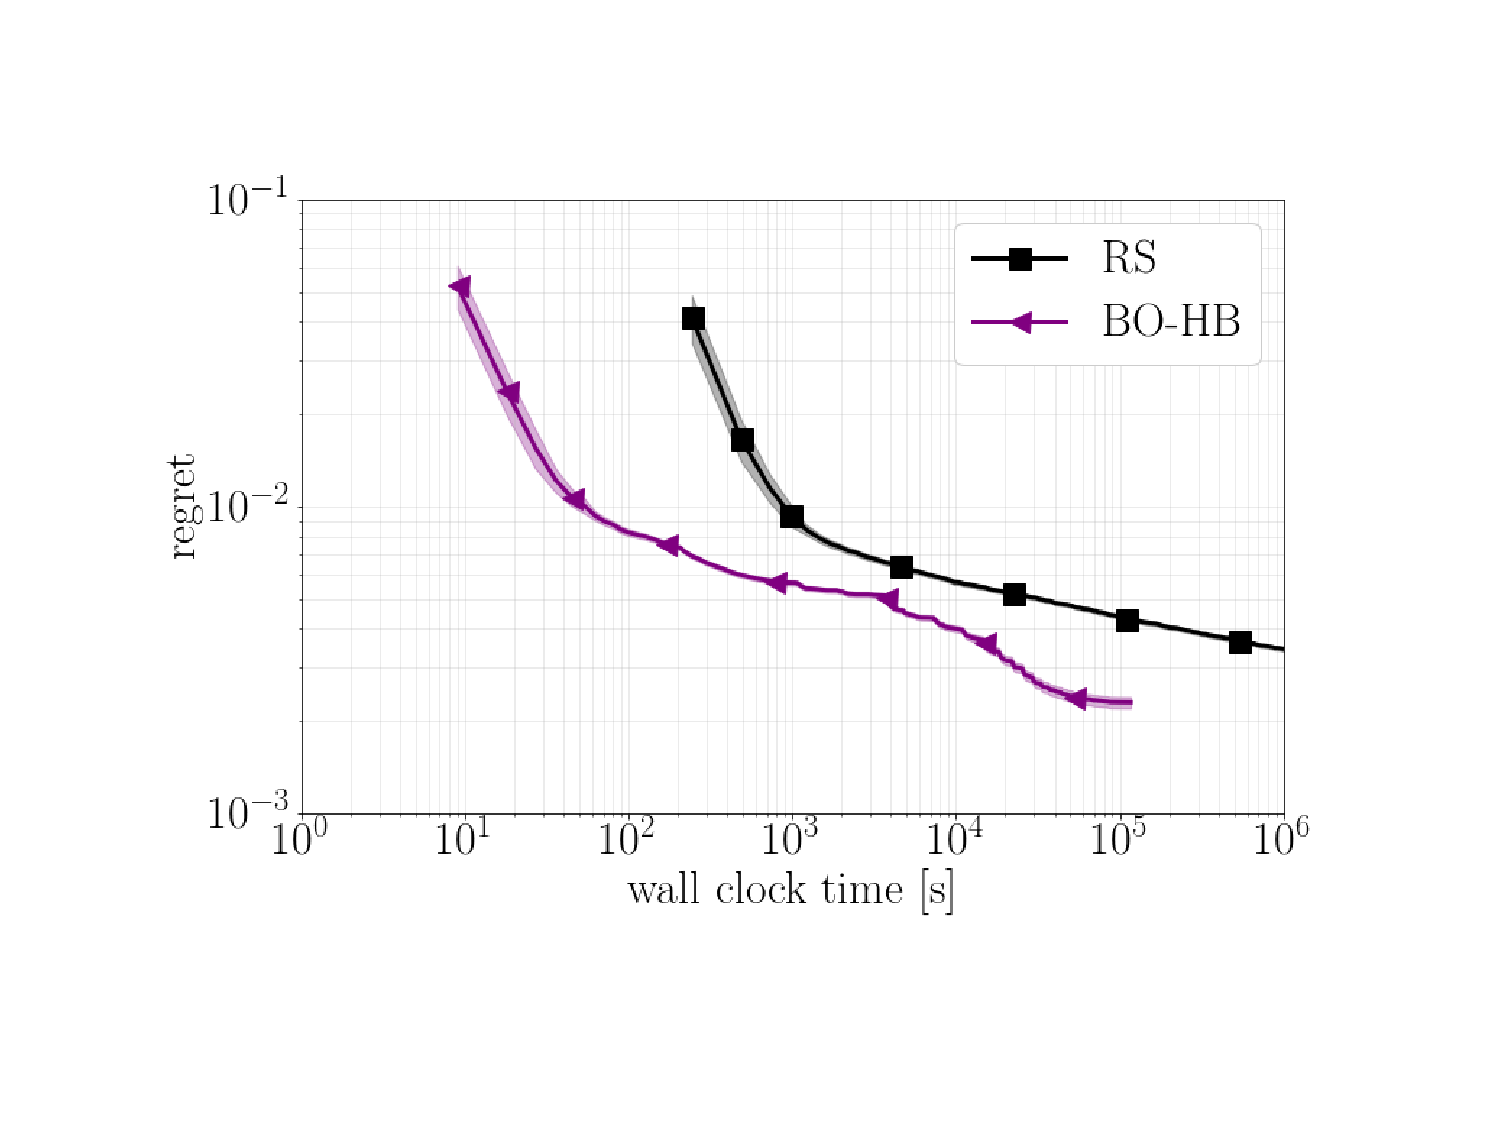
\includegraphics[width=0.65\textwidth]{../w07_hpo_speedup/images/bohb/BOHB_1.pdf}
    \caption{Performance of RS and BOHB on Auto-Net on dataset Adult}
\end{figure}

\end{frame}
%-----------------------------------------------------------------------
%----------------------------------------------------------------------
\begin{frame}{BOHB: Empirical Evaluation}
\begin{figure}
    \centering
    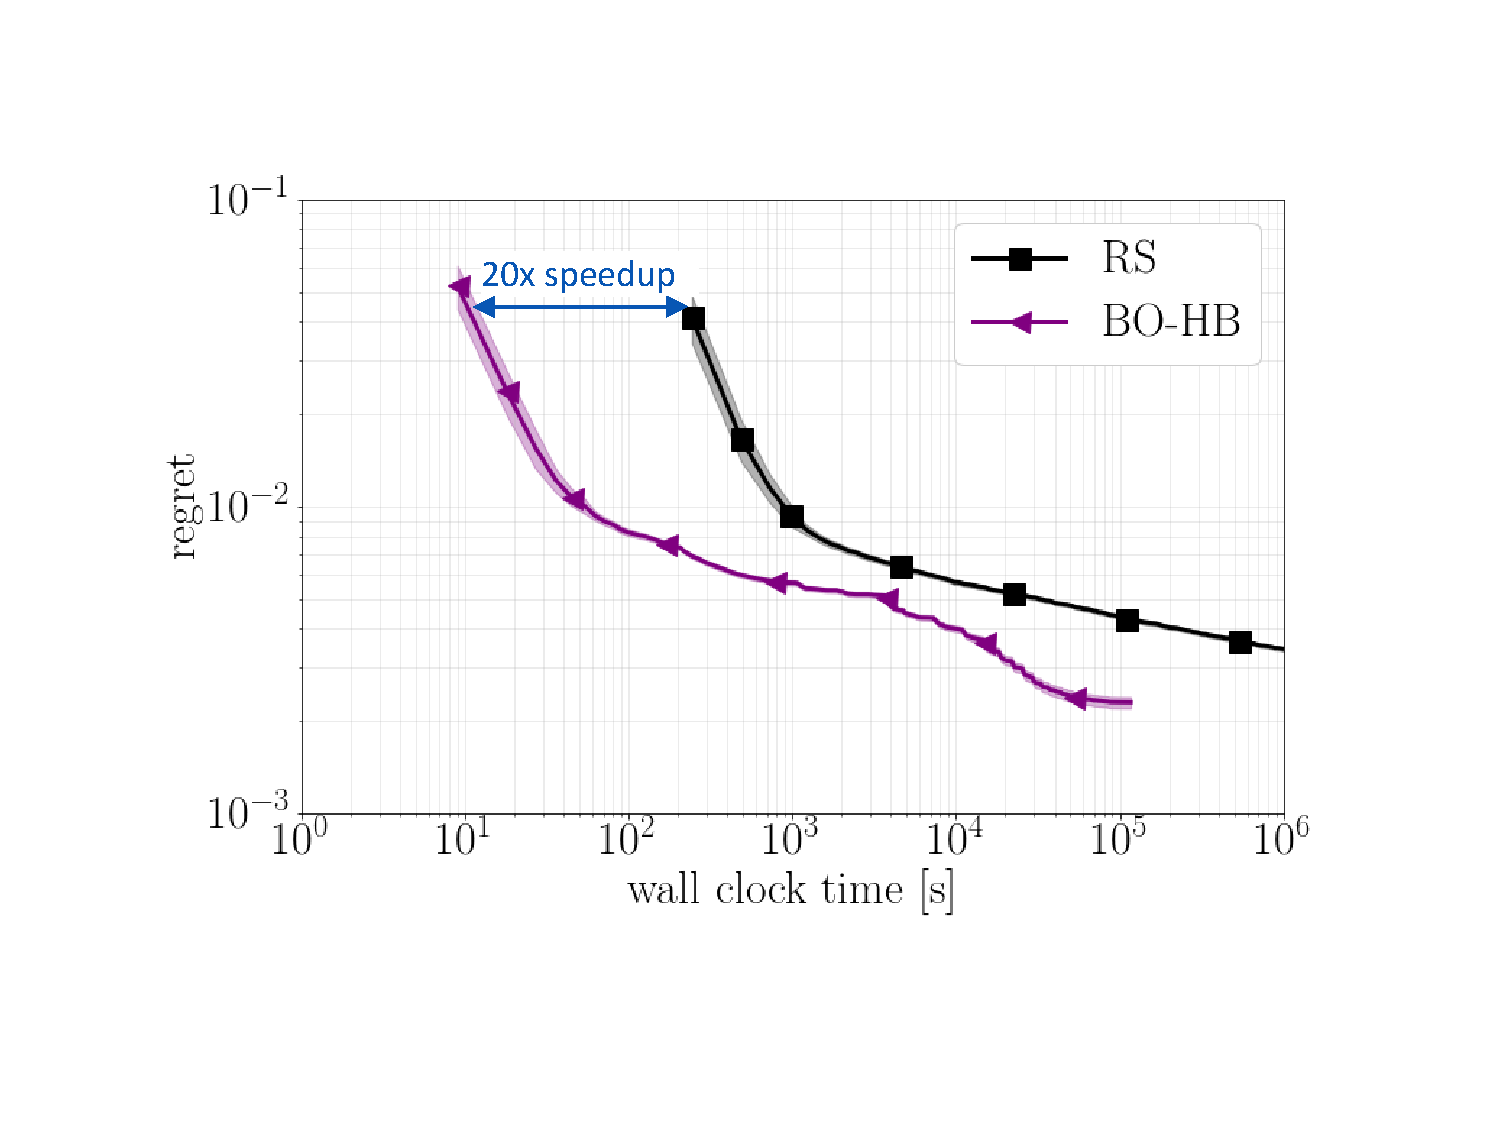
\includegraphics[width=0.65\textwidth]{../w07_hpo_speedup/images/bohb/BOHB_2.pdf}
    \caption{Performance of RS and BOHB on Auto-Net on dataset Adult}
\end{figure}

\end{frame}
%-----------------------------------------------------------------------
%----------------------------------------------------------------------
\begin{frame}{BOHB: Empirical Evaluation}
\begin{figure}
    \centering
    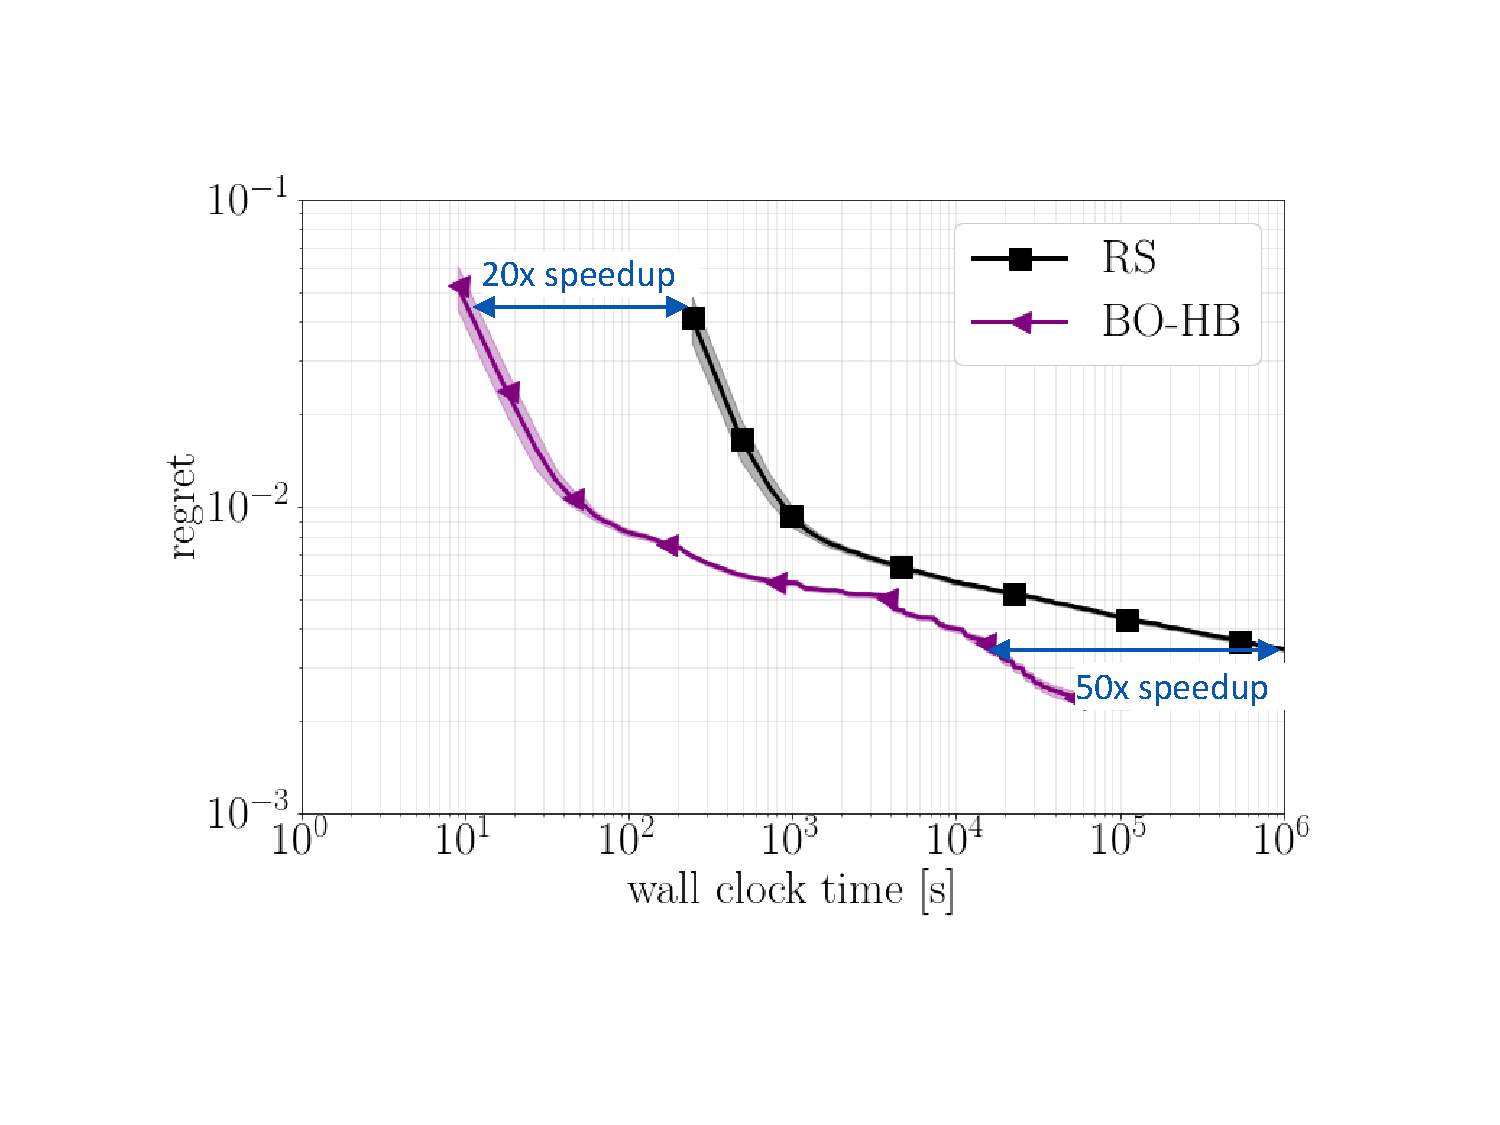
\includegraphics[width=0.65\textwidth]{../w07_hpo_speedup/images/bohb/BOHB_3.pdf}
    \caption{Performance of RS and BOHB on Auto-Net on dataset Adult}
\end{figure}

\end{frame}
%-----------------------------------------------------------------------
%----------------------------------------------------------------------
\begin{frame}{BOHB: Empirical Evaluation}
\begin{figure}
    \centering
    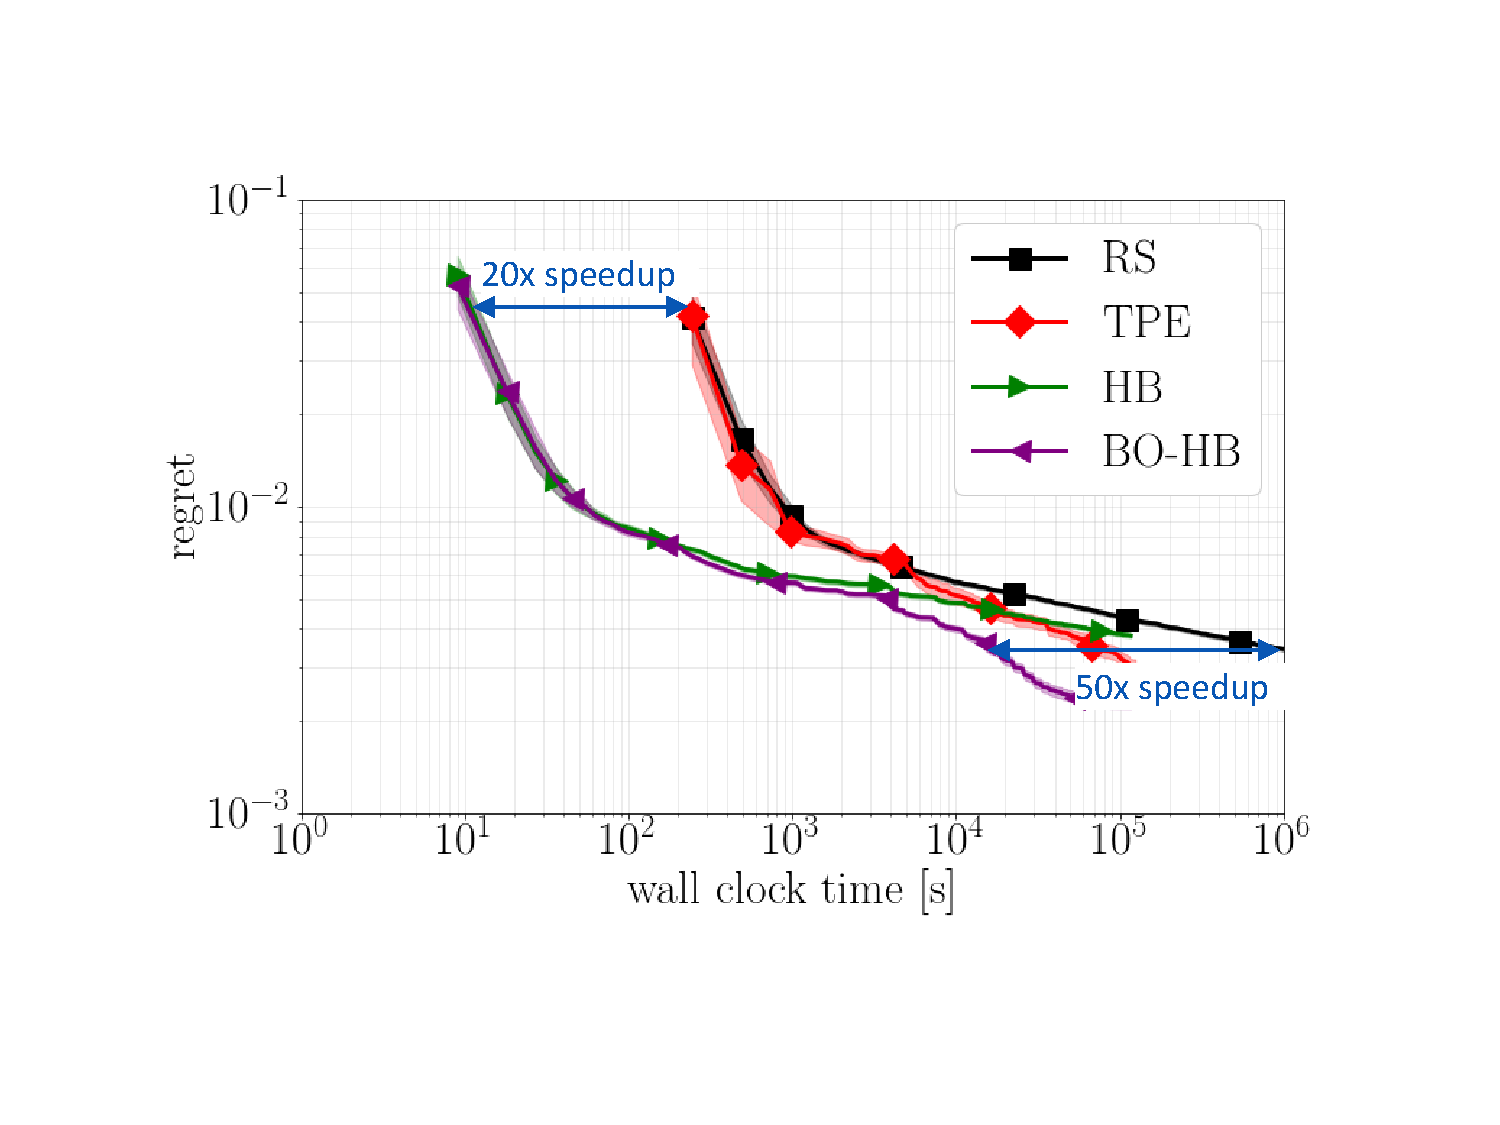
\includegraphics[width=0.65\textwidth]{../w07_hpo_speedup/images/bohb/BOHB_4.pdf}
    \caption{Performance of RS, TPE, HB and BOHB on Auto-Net on dataset Adult}
\end{figure}

\end{frame}
%-----------------------------------------------------------------------
%----------------------------------------------------------------------
\begin{frame}{BOHB: Different number of parallel workers}
\begin{figure}
    \centering
    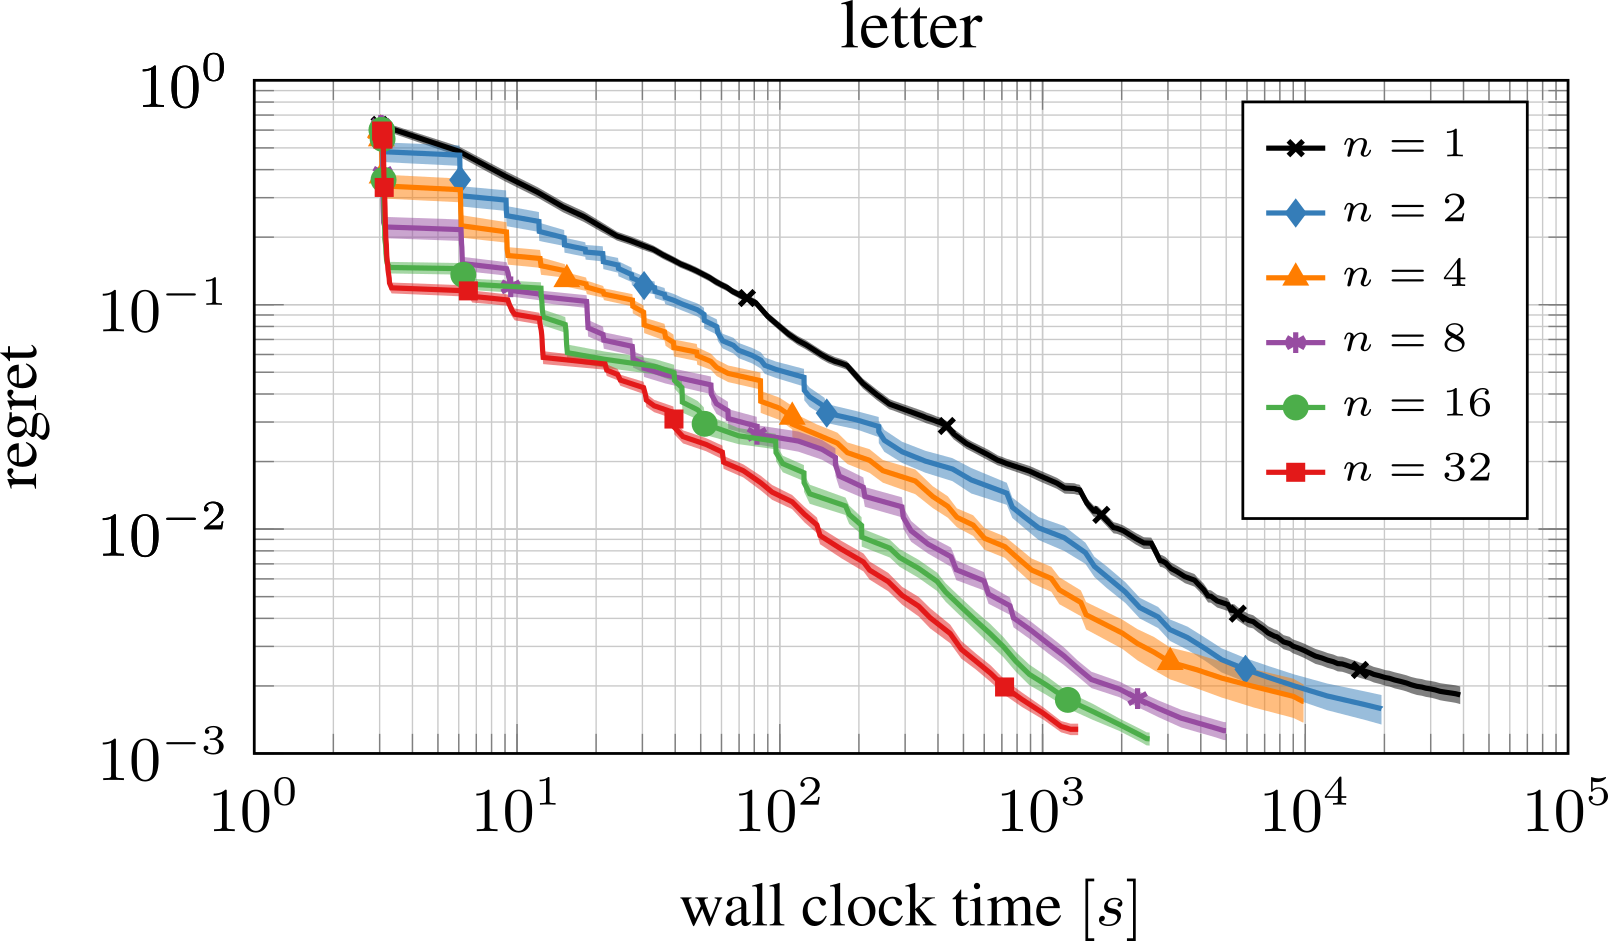
\includegraphics[width=0.65\textwidth]{../w07_hpo_speedup/images/bohb/parallelization_letter.png}
    \caption{Performance of BOHB with different number of parallel workers on the letter surrogate benchmark for 128 iterations}
\end{figure}

\end{frame}
%-----------------------------------------------------------------------
%----------------------------------------------------------------------
\begin{frame}{BOHB: Optimization of a Bayesian Neural Network}
\begin{figure}
    \centering
    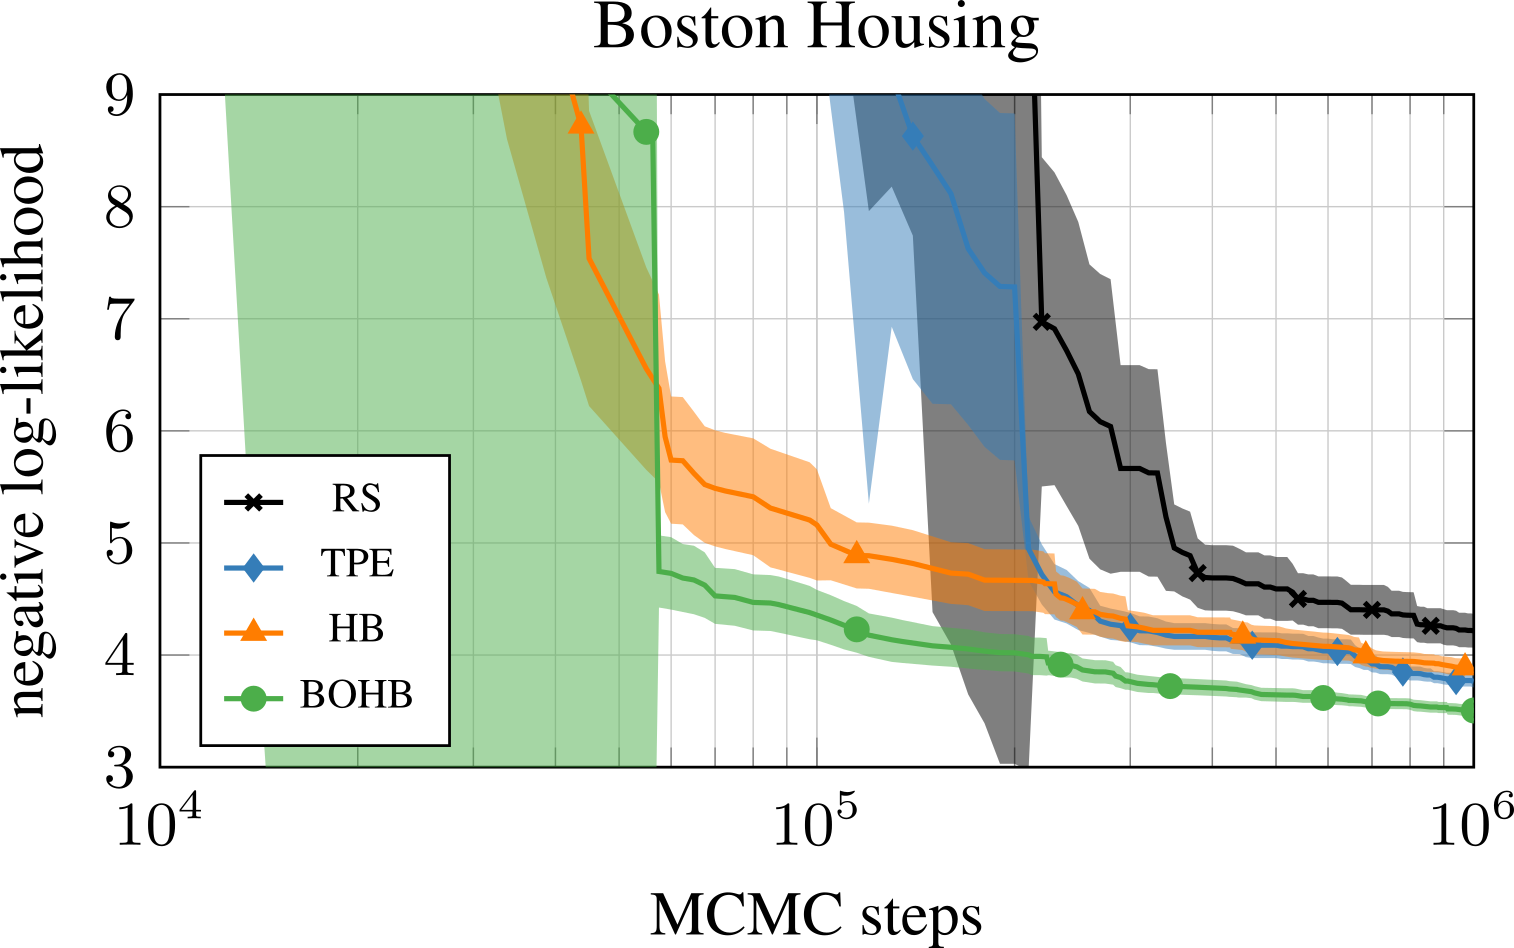
\includegraphics[width=0.65\textwidth]{../w07_hpo_speedup/images/bohb/bnn_boston-1.png}
    \caption{Optimization of 5 hyperparameters of a Bayesian neural network trained with SGHMC.}
\end{figure}

\end{frame}
%-----------------------------------------------------------------------
%----------------------------------------------------------------------
\begin{frame}{BOHB: Optimization of a Reinforcement Learning Agent}
\begin{figure}
    \centering
    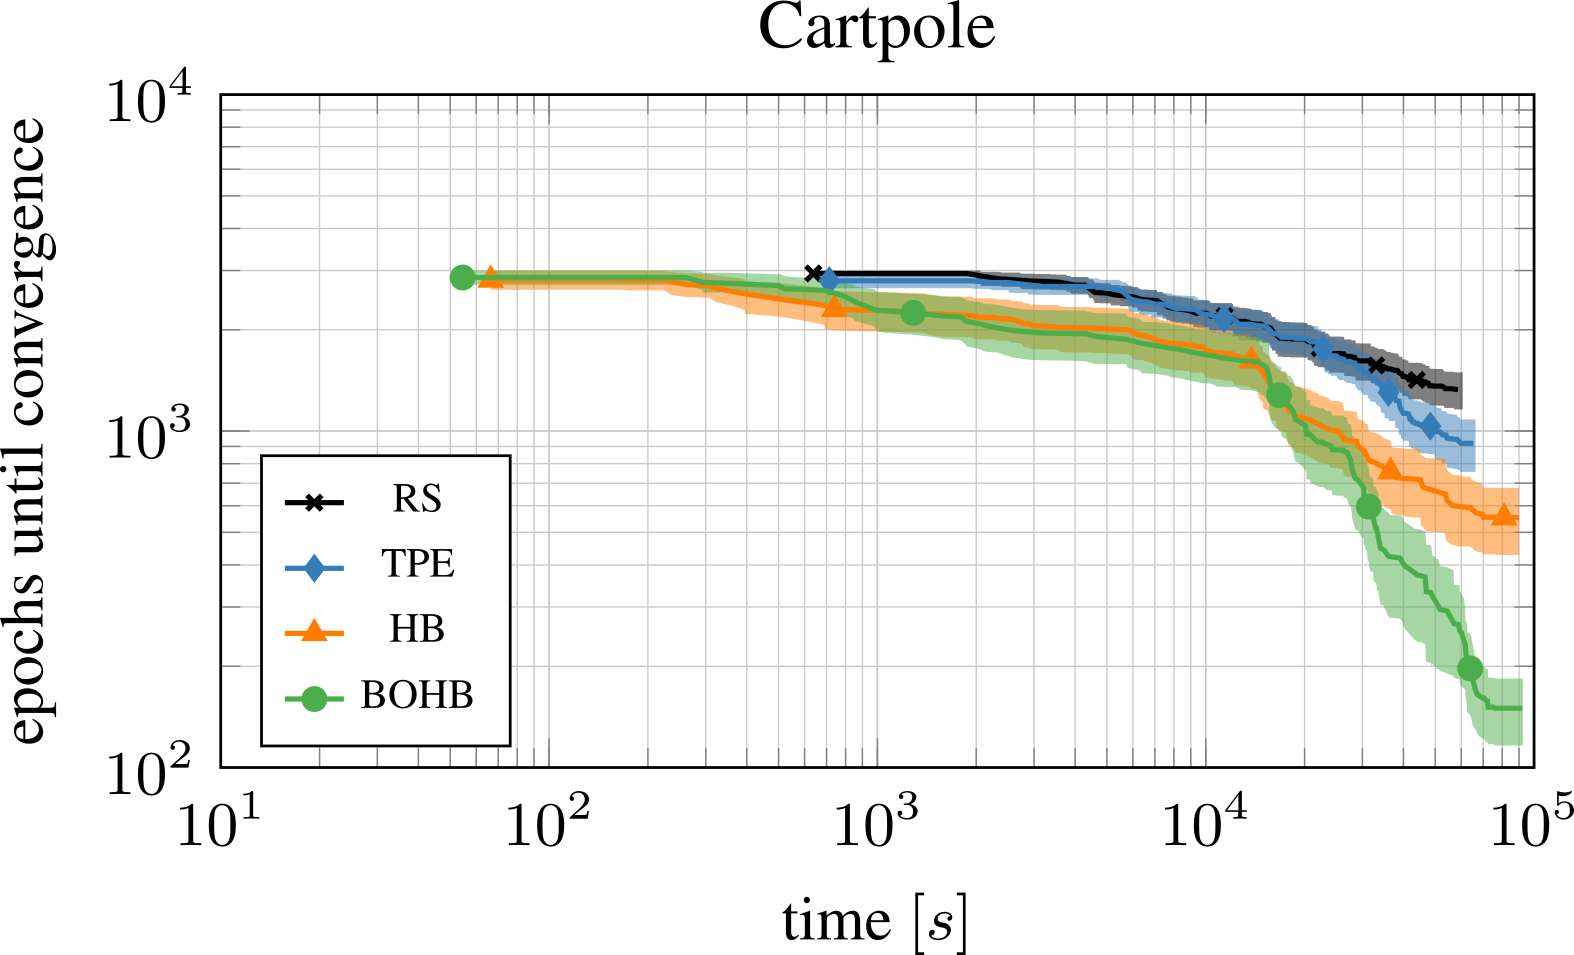
\includegraphics[width=0.70\textwidth]{../w07_hpo_speedup/images/bohb/cartpole-1.png}
    \caption{Hyperparameter optimization of 8 hyperparameters of PPO on the cartpole task.}
\end{figure}

\end{frame}
%-----------------------------------------------------------------------
%----------------------------------------------------------------------
\begin{frame}{BOHB: Optimization of an SVM}
\begin{figure}
    \centering
    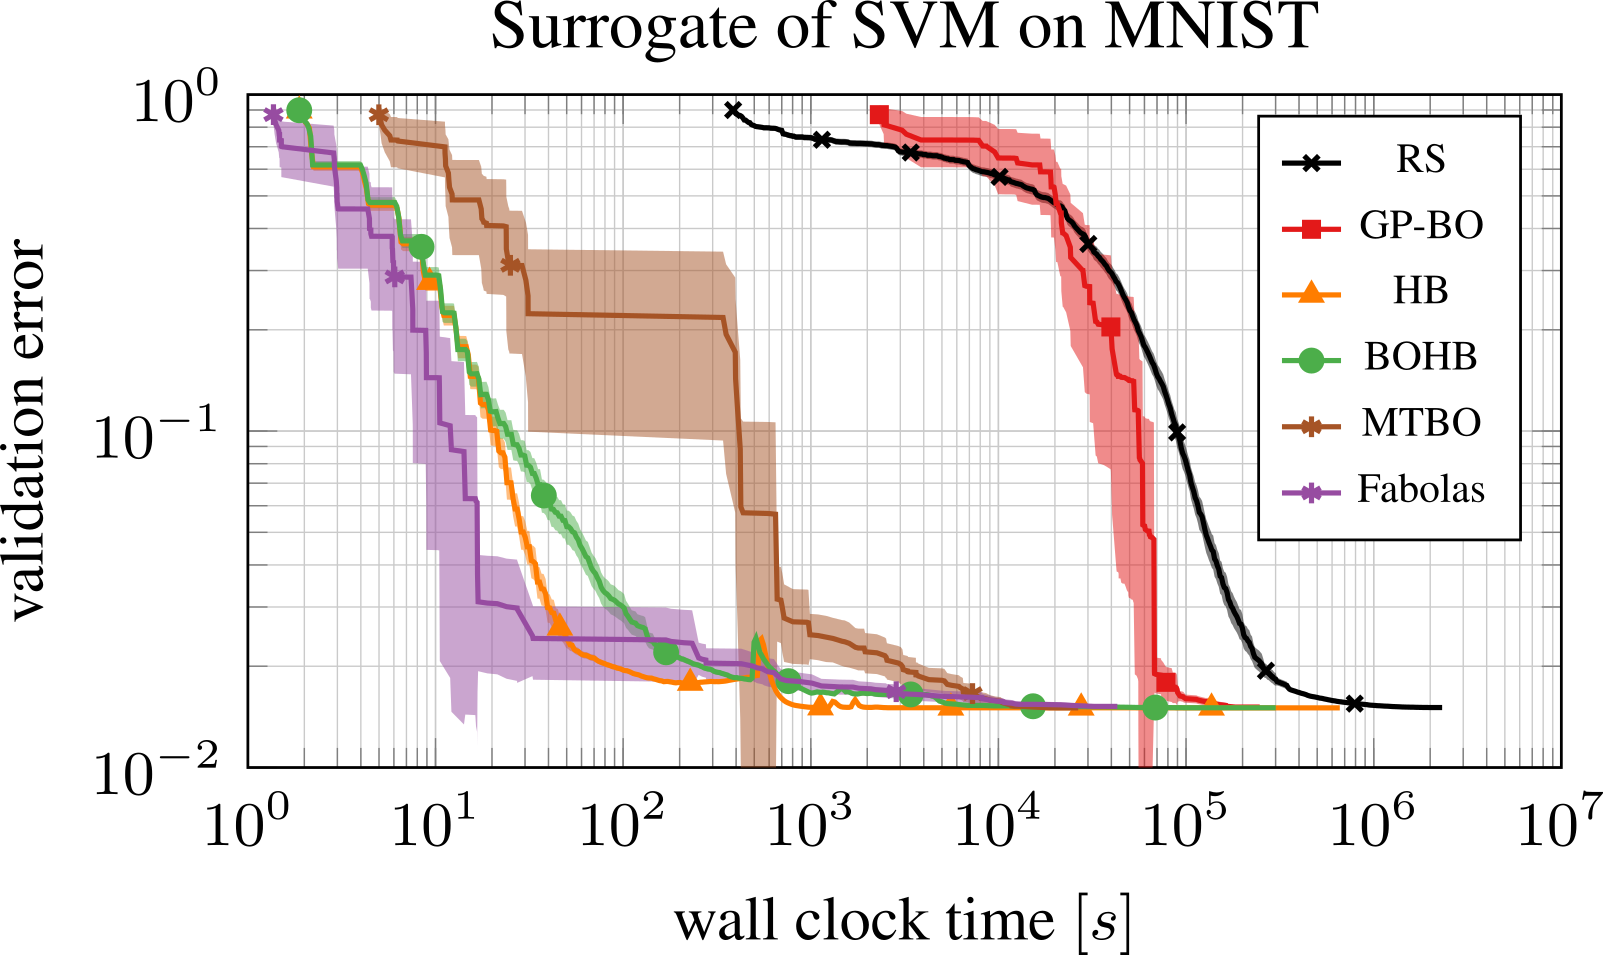
\includegraphics[width=0.70\textwidth]{../w07_hpo_speedup/images/bohb/svm_surrogate_test_pdf-1.png}
    \caption{Comparison on the SVM on MNIST surrogate benchmark}
\end{figure}

\end{frame}
%-----------------------------------------------------------------------
%----------------------------------------------------------------------
\begin{frame}{BOHB: Counting Ones }
\begin{figure}
    \centering
    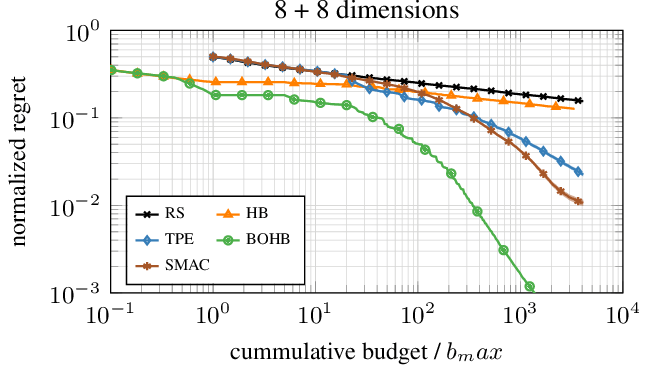
\includegraphics[width=0.70\textwidth]{../w07_hpo_speedup/images/bohb/countingones_bohb.png}
    \caption{Results for the counting ones problem in 16 dimensional
space with 8 categorical and 8 continuous hyperparameters.}
\end{figure}

\end{frame}
%-----------------------------------------------------------------------
%----------------------------------------------------------------------
\begin{frame}{BOHB: Optimization of a Feedforward Network}
\begin{figure}
\vspace*{-0.2cm}
    \centering
    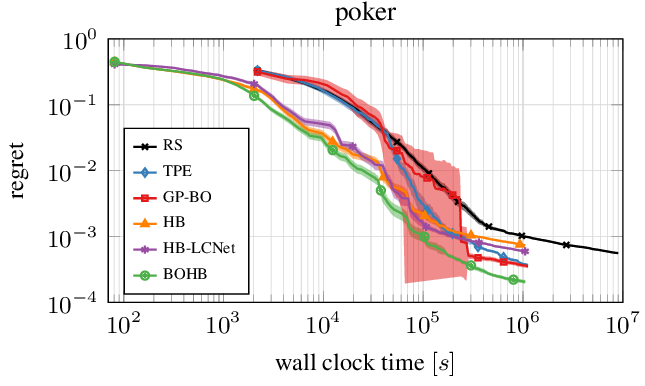
\includegraphics[width=0.70\textwidth]{../w07_hpo_speedup/images/bohb/surrogate_on_poker.png}
    \caption{Optimizing six hyperparameters of a feed-forward neural
network on featurized datasets; results are based on surrogate
benchmarks. }
\end{figure}

\end{frame}
%-----------------------------------------------------------------------

%-----------------------------------------------------------------------
\begin{frame}{Questions to Answer for Yourself / Discuss with Friends}

\bigskip

\begin{itemize}
    \item \alert{Repetition.} Why does BOHB interleave randomly sampled configurations in the optimization process?

\medskip
    \item \alert{Discussion.} 
    What are the advantages of the Parzen estimator model over more advanced models such as random forests or Gaussian processes?

\end{itemize}

\end{frame}
%----------------------------------------------------------------------
%----------------------------------------------------------------------